\documentclass[11pt, oneside]{article} 
\usepackage{geometry}
\geometry{letterpaper} 
\usepackage{graphicx}
	
\usepackage{amssymb}
\usepackage{amsmath}
\usepackage{parskip}
\usepackage{color}
\usepackage{hyperref}

\graphicspath{{/Users/telliott/Dropbox/Github-Math/figures/}
{figures/}}

\title{Pentagon}
\date{}

\begin{document}
\maketitle
\Large

%[my-super-duper-separator]

By the standard definition, a pentagon is a polygon having five equal sides.  However, the pentagon can also be defined as being formed by five evenly spaced points on a circle, with five equal central angles that total four right angles.
\begin{center} 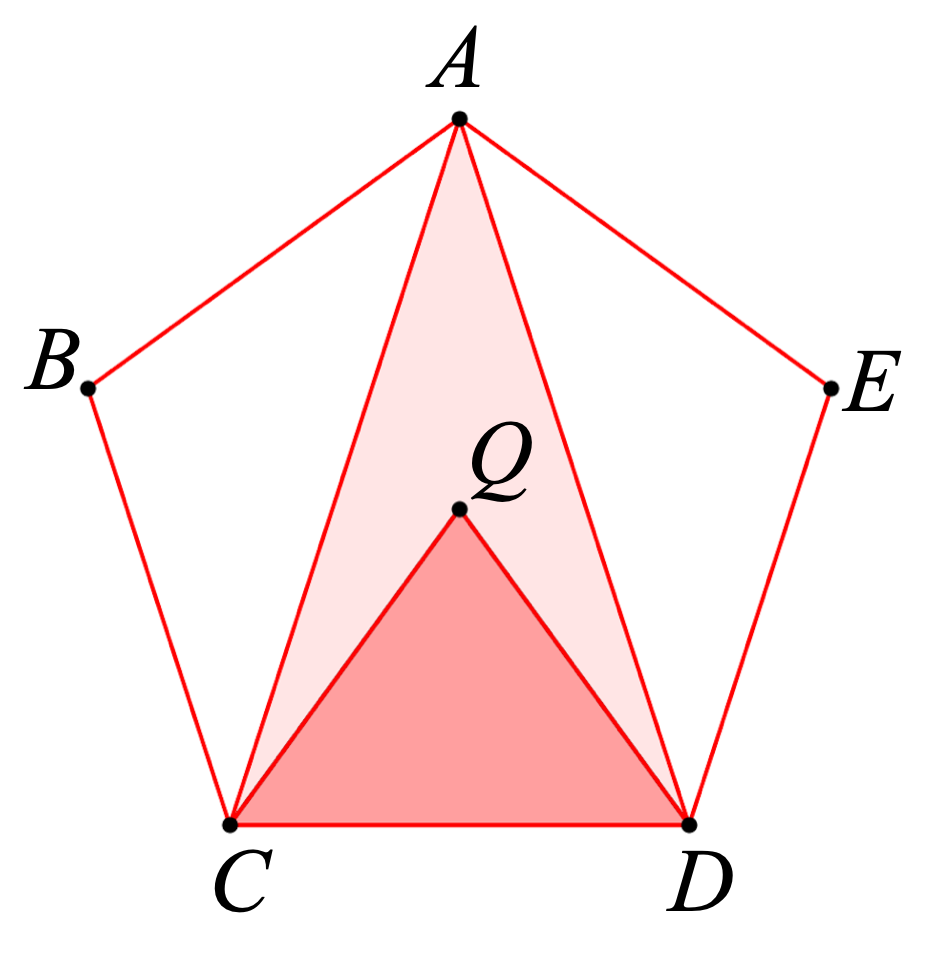
\includegraphics [scale=0.3] {pent_central_label.png} \end{center}

Either way, we will need more insight if we wish to construct a pentagon.

Since there are five triangles like $\triangle QCD$, the central angles are each $1/5$ of the whole circle, or 2/5 of a triangle, $72^\circ$ in modern notation.  By the inscribed angle theorem, $\angle CAD$ with the same endpoints has one-half the measure, 1/5 of a triangle.  

We claim that $\triangle ACD$ is isosceles, thus, the base angles are twice the vertex angle, in the overall ratio 1:2:2.  

\emph{Proof}.  

Since the five triangles like $\triangle QCD$ have the same central angle and the same arms, they are all congruent by SAS.  It follows that the total angles at the vertices $A,B \dots$, such as $\angle BCD$  are all equal and twice the base angles of $\triangle QCD$ such as $\angle QCD$.  

\begin{center} 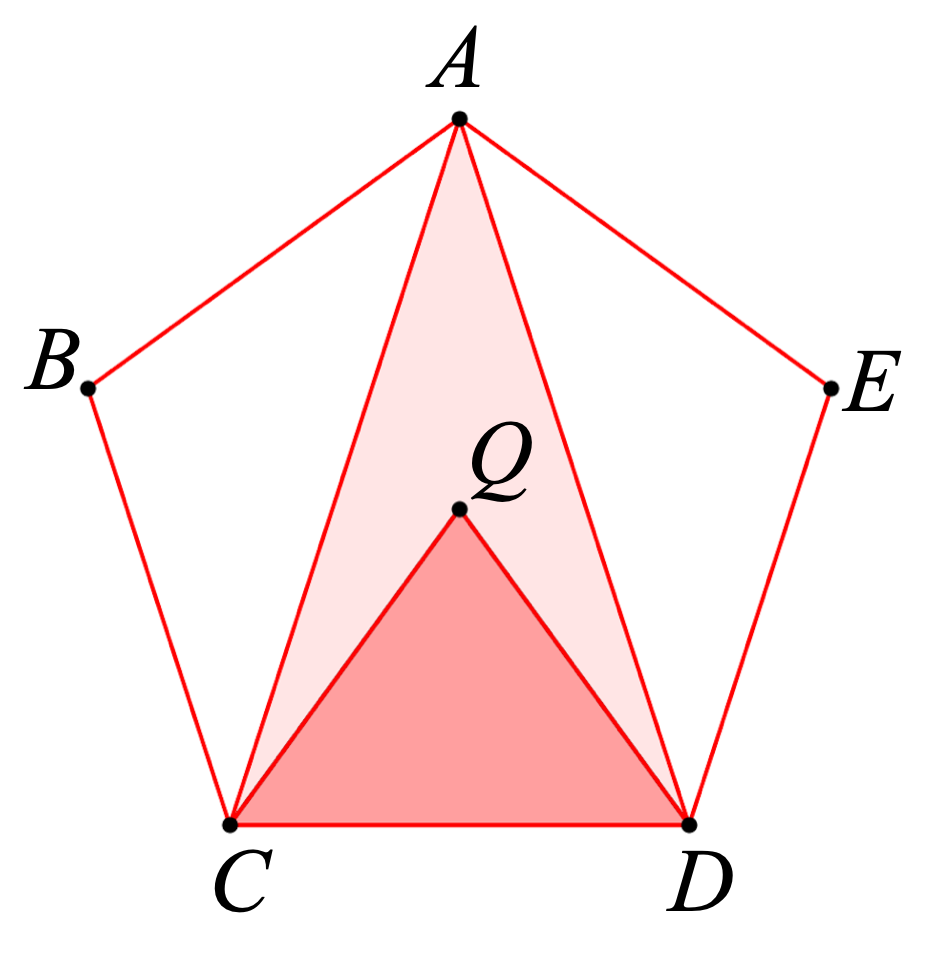
\includegraphics [scale=0.3] {pent_central_label.png} \end{center}

Then $\triangle ABC \cong \triangle AED$ by SAS.  By subtraction, the base  $\angle ACD = \angle ADC$ and $AC = AD$ by I.6.  

$\square$

 As a result, we have $4/5$ of two right angles to be divided equally for the base angles of the isosceles $\triangle ACD$.

\subsection*{IV.10}

Euclid shows how to construct such a triangle in IV.10.

\begin{center} 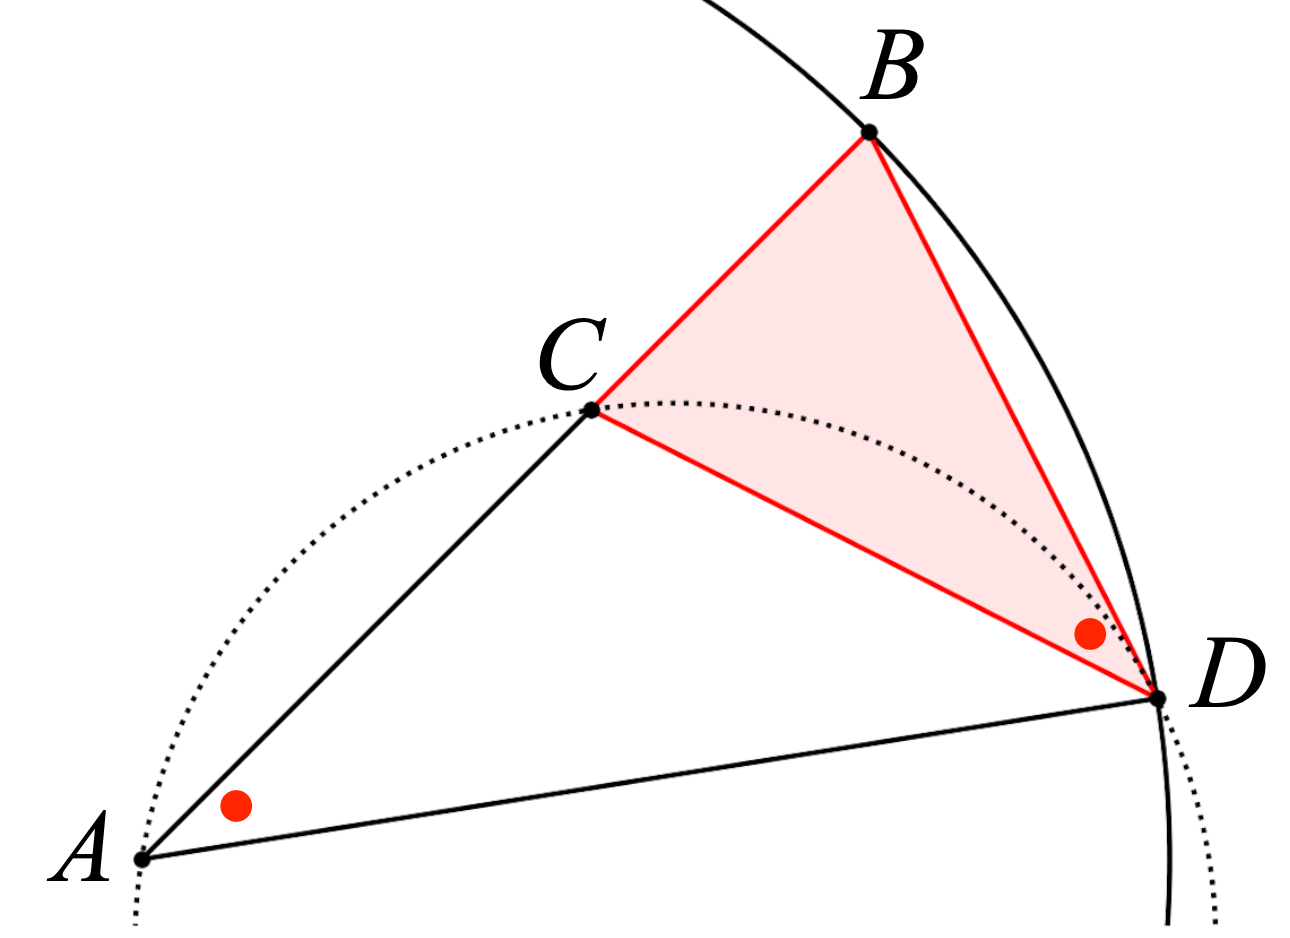
\includegraphics [scale=0.3] {EIV_10_label.png} \end{center}

Briefly, point $C$ is placed so that $AB/AC = AC/BC$;  $D$ is placed on the circle on center $A$ with radius $AB$, such that the length $BD = AC$.  We can use the converse of the tangent-secant theorem to show that $BD$ is tangent to the circle containing $ACD$, and then $\angle BDC = \angle BAD$.  

Then since $\triangle ACD$ is isosceles, $\angle ADC = \angle DAC$, so $\angle ADB$ is bisected.  But $\triangle ABD$ is isosceles, so the two equal base angles are each twice the entral angle at $A$. 

\subsection*{continuation}

\begin{center} 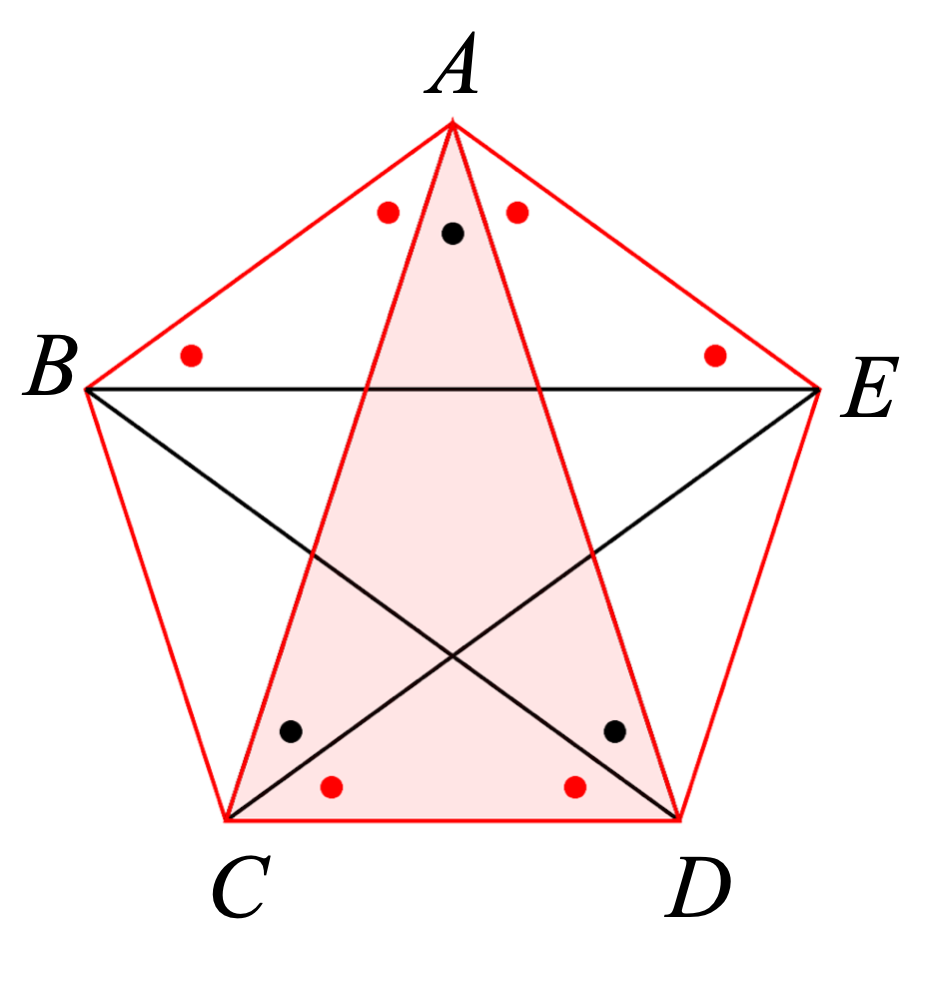
\includegraphics [scale=0.4] {pent2_label.png} \end{center}

Going back to the first diagram, we can show that $\angle CAD$ is one-third the total angle at the vertex $A$.  Since the flanking angles are equal, together $AC$ and $AD$ form three equal angles at vertex $A$.

\emph{Proof}.  We might count fractions of a right angle.  Another approach is to use the triangle sum theorem.  We showed that the base angles of $\triangle BAC$ are equal.  Let them equal $x$ (red dots).  Let the angles like $\angle CAD$ have measure $y$ (black dots).  Then in $\triangle ABE$ we have $4x + y$ and in $\triangle ACD$ we have $3x + 2y$.  Since these sums are equal, it follows that $x = y$.  $\square$

\begin{center} 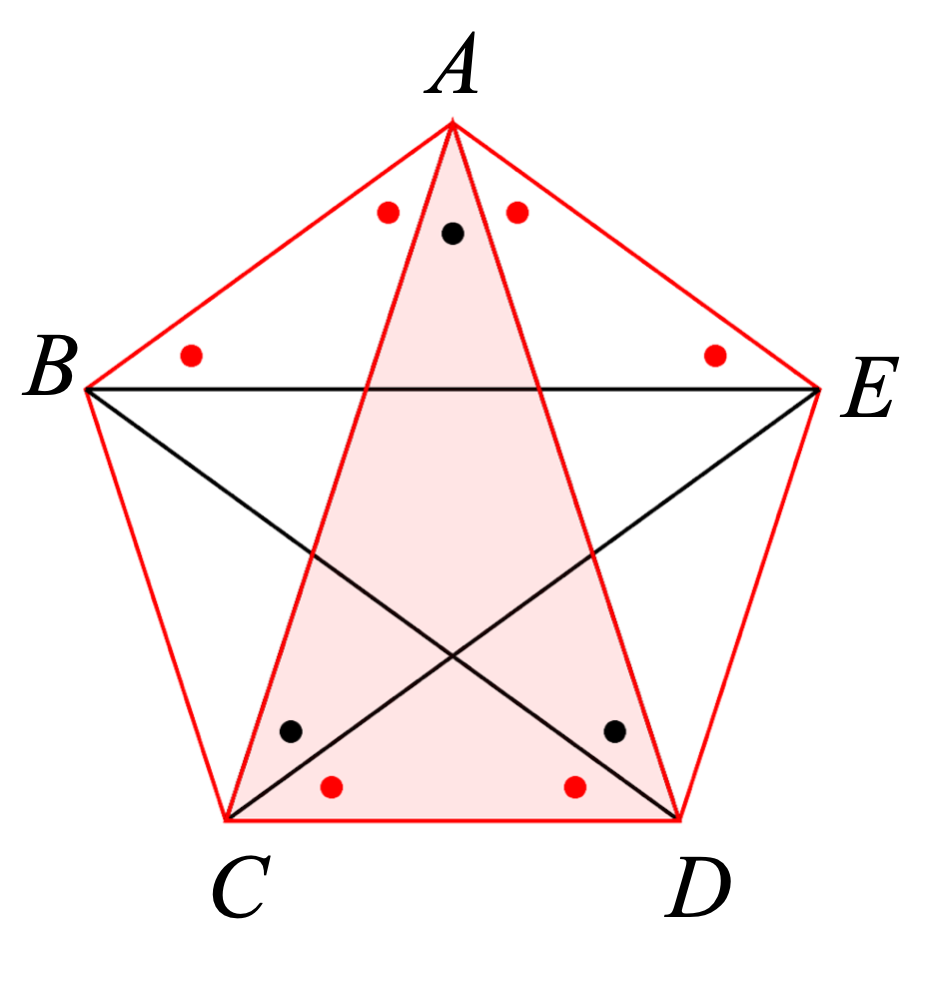
\includegraphics [scale=0.4] {pent2_label.png} \end{center}

As a result, we have that the base angles of $\triangle ACD$ have the same measure as the central angle $QCD$ in the first figure.  We also have that $\angle A$ plus $\angle ABD$ is equal to two right angles, so $AE \parallel BD$, $AB \parallel CE$, $ABXD$ is a rhombus (parallelogram), and the inner figure is a regular pentagon.

In $\triangle ACD$, the ratio of the long sides to the base is the same as the golden ratio or mean, usually called $\phi$, as defined by Euclid's construct above.

\begin{center} 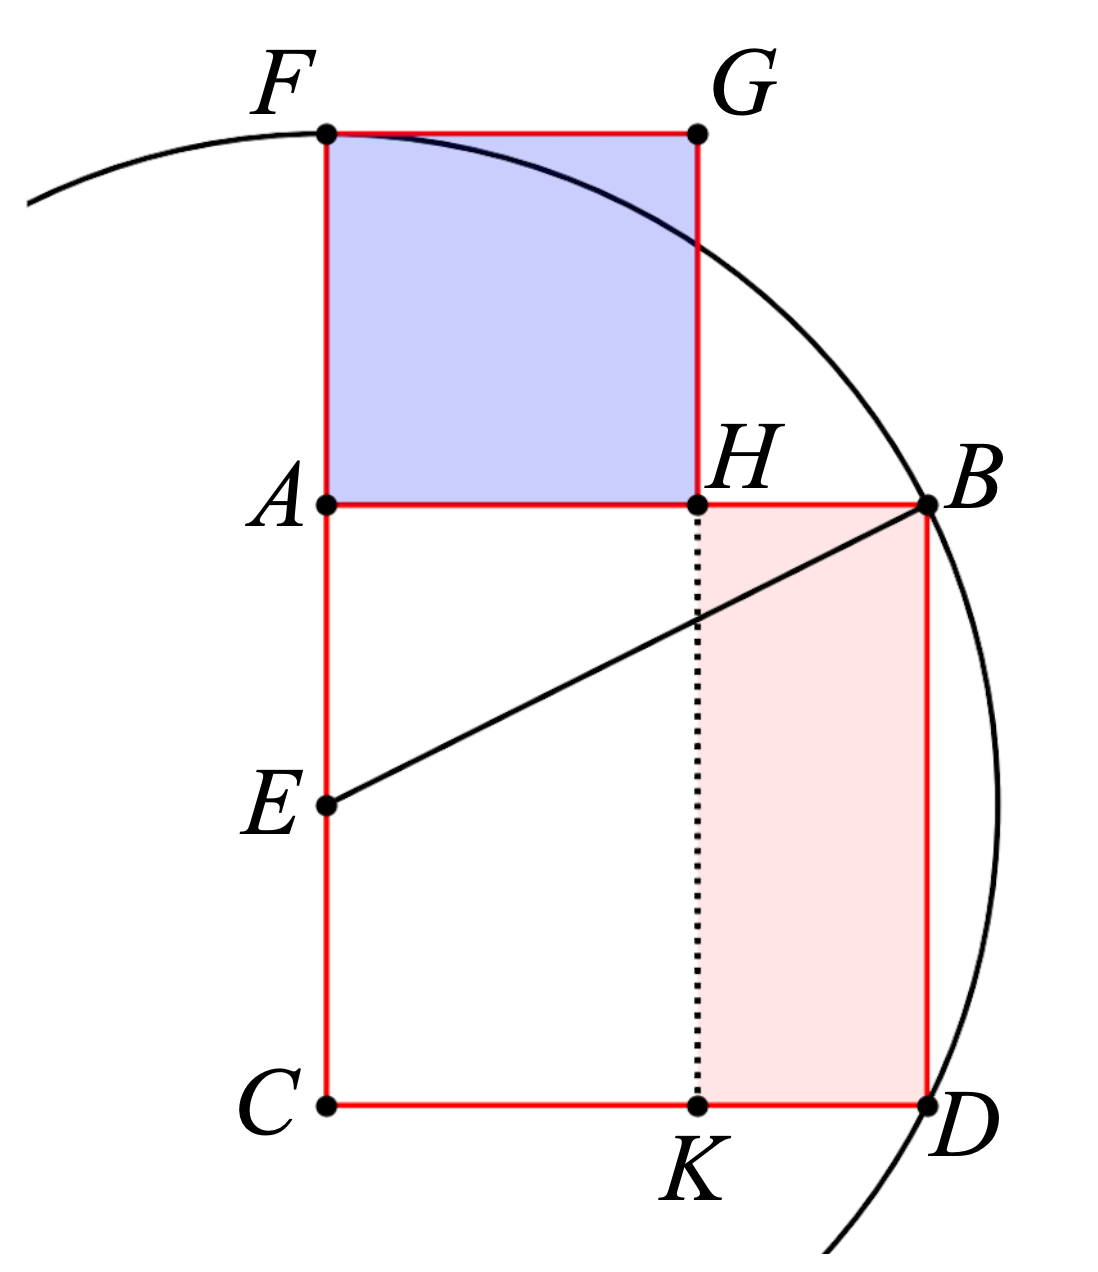
\includegraphics [scale=0.3] {EII_11_label.png} \end{center}

Go back to the construction of the golden ratio in EII.11.  If $AE$ has length $1$, then $BE = EF$ has length $\sqrt{5}$.  $AH = AF$ has length $\sqrt{5}-1$.  $AB/AH = \phi = 2/(\sqrt{5}-1)$.  Rationalizing the denominator we have
\[ \phi = \frac{2}{\sqrt{5}-1} \cdot \frac{\sqrt{5}+1}{\sqrt{5}+1} = \frac{\sqrt{5}+1}{2}  \]

\begin{center} 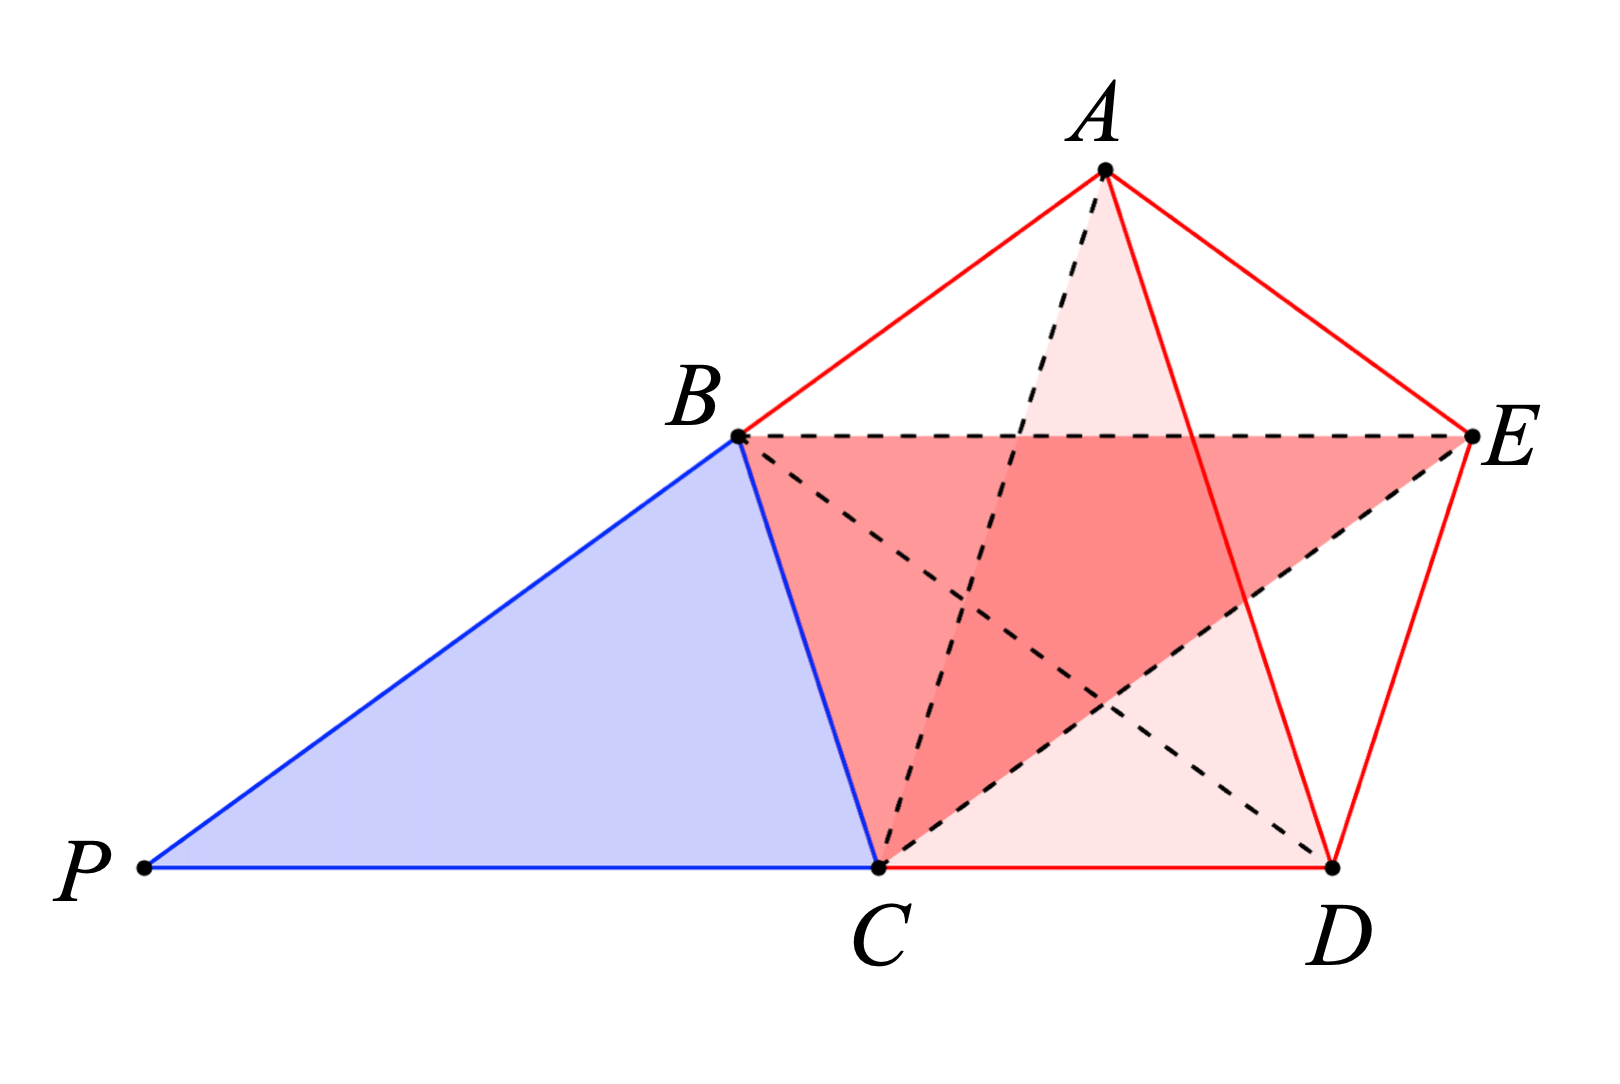
\includegraphics [scale=0.3] {easy_pent_label.png} \end{center}

In the figure above $\triangle PBC \cong \triangle ACD$.  \emph{Proof}.  $\triangle PAB$ is similar to both, and they have equal bases.  $\square$

Then the ratio of one-half of $BC$ to $PB$ is $1/2$ divided by $\phi$ or $1/2\phi$.  This is the cosine of $\angle PCB = \angle ACD = 72^\circ$, the same as the central $\angle CQD$.

We also have that the length of $BE$ is $\phi/2$, but this same length divided by the unit side length gives the cosine of $\angle ABE = 36^\circ$.

We can use these results to verify the correctness of the next method for construction of a pentagon.
\begin{center} 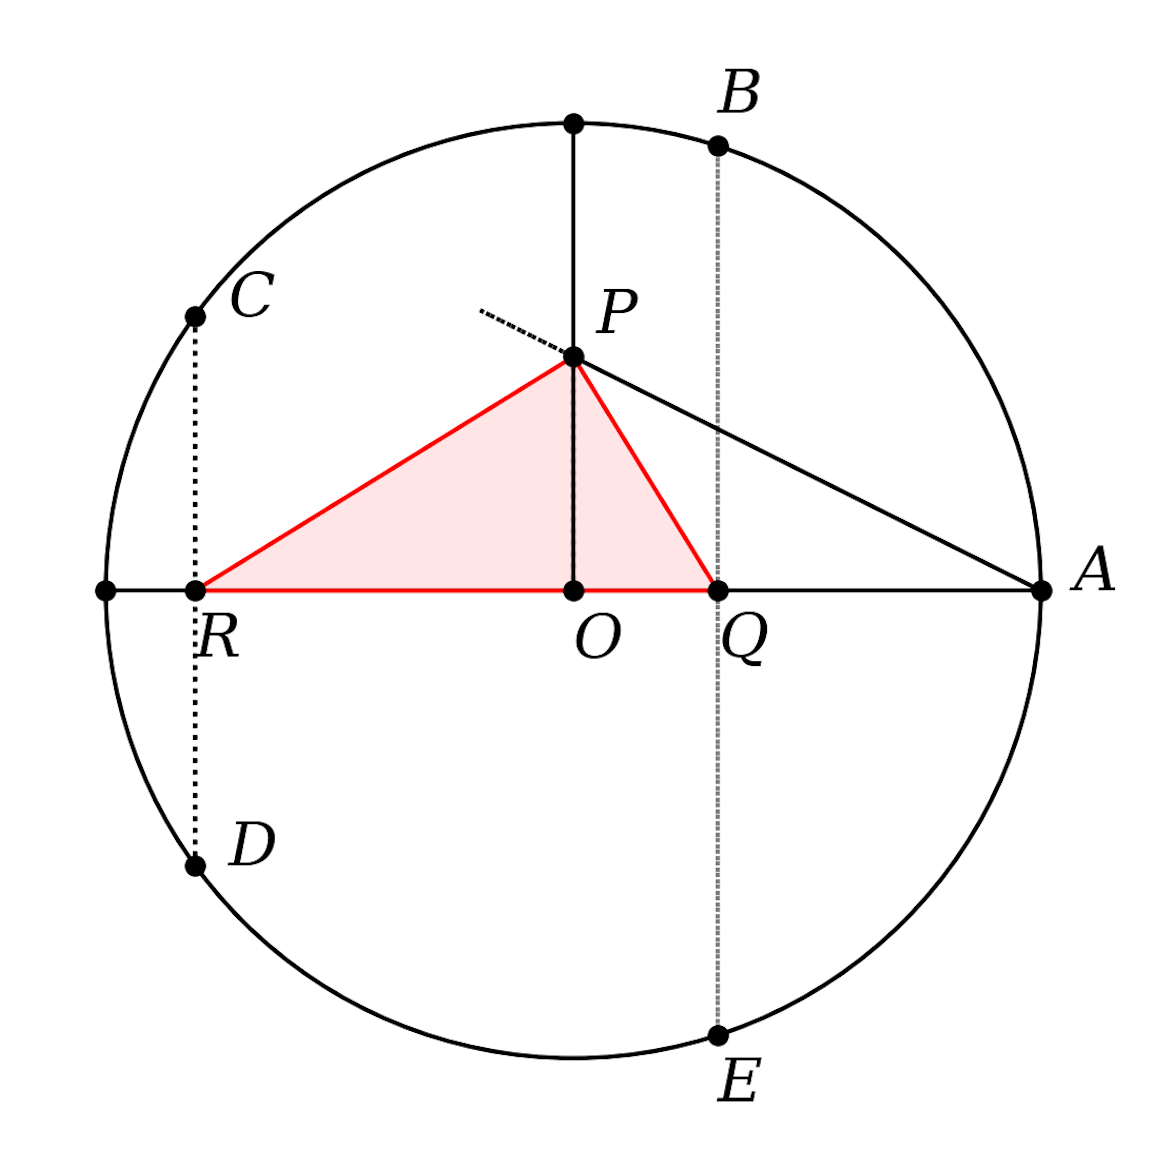
\includegraphics [scale=0.4] {basic_pentagon_crop.png} \end{center}

Let the radius $AO$ be $2$, bisected at $P$, so $AP = \sqrt{5}$.  Bisect $\angle OPA$, then $AQ/OQ = \sqrt{5}$.  

So $AQ + OQ = (1+\sqrt{5}) \cdot OQ = 2$.  Thus $OQ = 1/\phi$.

$OQ/OB = 1/2\phi$ and so $\angle BOA$ is equal to the central angle in a pentagon constructed on this circle.

Finally, draw the right $\triangle QPR$.  $OP^2 = 1$ and this is equal to $OQ \cdot OR$.  Thus $OR$ equals $\phi$, which gives $\phi/2$ as the cosine of $\angle COR$ which is $36^\circ$.

We have the following values for cosine:
\[ \cos 36 = \frac{\phi}{2} \ \ \ \ \ \ \  \cos 72 = \frac{1}{2 \phi}  \]

We can get more values from the Pythagorean theorem, the definition ($\phi^2 = \phi + 1)$, and from the double angle formula.  For example:
\[ \sin^2 36 = 1 - \frac{\phi^2}{4}  = \frac{4 - \phi - 1}{4} \]
\[ \sin 36 = \frac{\sqrt{3 - \phi}}{2} \]
and
\[ \sin 72 = 2 \sin 36 \cos 36 =  2  \frac{\sqrt{3 - \phi}}{2} \cdot \frac{\phi}{2}  \]
\[ \sin^2 72 = \frac{(3-\phi)(\phi + 1)}{4} = \frac{3 + 2 \phi - (\phi + 1)}{4}\]
\[ = \frac{\phi + 2}{4} \]
\[ \sin 72 = \frac{\sqrt{2 + \phi}}{2} \]

which can be checked
\[ \frac{2 + \phi}{4} + \frac{1}{4 \phi^2} = \frac{2 \phi^2 + \phi^3 + 1}{4 \phi^2} \]
The numerator is
\[ 2 \phi + 2 + (\phi + 1)\phi + 1 = 4 \phi + 4 \]
which is equal to the denominator.  We satisfy the identity $\sin^2 \theta + \cos^2 \theta = 1$.

Of course, now that we know sine and cosine of $36^\circ$ and $72^\circ$, we also know them for $18^\circ$ and $54^\circ$.

\subsection*{ratio of sines}

We can also say something about the ratio of two sines.  Recall that the ratio of the chord of a regular pentagon to the side is equal to $\phi$.

Considered as part of the circumcircle, the side is a chord as well, of the circumcircle.  Using the standard result that the chord is the diameter times the sine of the angle, we have that
\[ \frac{\sin 72^\circ}{\sin 36^\circ} = \frac{\phi}{1} = \phi \]

Plugging in the values from our work above, we must have that
\[ \phi = \frac{\sqrt{2 + \phi}}{\sqrt{3 - \phi}} \]

which seems hard to believe.  Let us work backward.  Square and rearrange:
\[ \phi^2 \cdot (3 - \phi)= (2 + \phi) \]
Working with the left-hand side:
\[ (\phi + 1)(3 - \phi) = 2 \phi + 3 -  \phi - 1 = 2 + \phi \]
which is correct.

\subsection*{radius}

Another important question is the radius of the circle that circumscribes the pentagon.  Returning to the central angle, observe that

\begin{center} 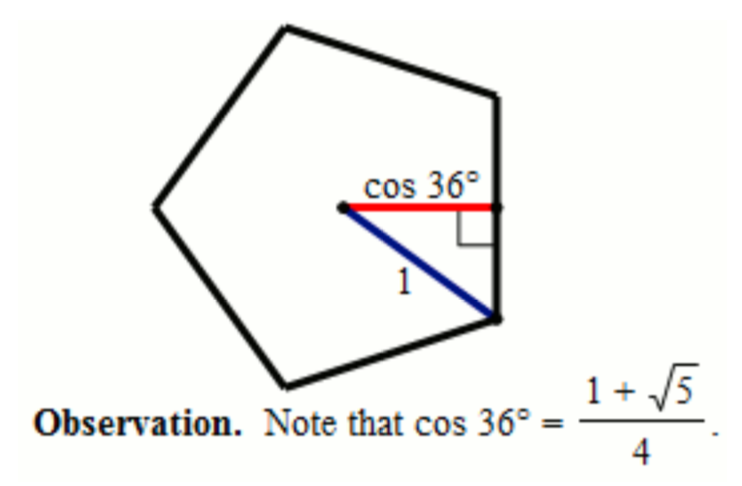
\includegraphics [scale=0.3] {cos36.png} \end{center}

If the side length is $s$ then the half side is $s/2$ and $s/2r$ is the sine of the central angle, $\sin 36^\circ$ so the ratio is
\[ \frac{s}{r} = 2 \sin 36 = \sqrt{3 - \phi} = \sqrt{\frac{5 - \sqrt{5}}{2}}  \]

\end{document}